\section*{Introduction}

%This work deals with the development of a controller able to suppress the vibration and unwanted inputs in a bilateral control system.

Teleoperation extends the human capability to manipulating objects remotely. An important aspect deals with necessity to obtain, on operator side, similar condition as those at the remote location, in other words, a proper feedback. 

A bilateral system is composed by a joystick, called \emph{master}, on the human side, connected to a \emph{slave} on the environment side.

The human imposes a force on the master, that results in a displacement. This displacement is then transmitted to the slave. On the other side, the slave has a force sensor used to "send back" to the master the reflection forces at the environment side. For these reasons we can call it \emph{bilateral teleoperation}.

Two important goals of the teleoperation are \cite{hokayem2006bilateral}:
\begin{itemize}
	\item \textbf{Stability} of the closed loop system irrespective to the behavior of the human and the environment;
	\item \textbf{Transparency} of the teleoperation task: we want forces and displacements be the same on the two sides of the system. 
\end{itemize}

Stability of the system can be ruined by unwanted disturbance, internal and external:
\begin{itemize}
	\item \textbf{Internal disturbance}, due to the uncertainties in modeling of the system;
	\item \textbf{External disturbance}, such as unexpected input contaminated with vibration noise from both sides og the system.
\end{itemize}

This report deals with the development of a controller able to suppress the vibration and unwanted inputs in a bilateral control system \cite{trakarnchaiyo2017vibration}.

In particular, the work is based on the concept of one degree of freedom inertia-spring-damper system. This concept comes from the design of shock absorbers used in vehicle suspension (which is composed by a spring and damper), and is usually applied in bilateral control system for \emph{soft manipulation}.

In this work we investigate the concept of \textit{virtual} spring-damper system with an additional inertia.
The disturbance suppression performances depends on the value of these virtual parameters, determined from the desired cut-off frequencies.

The report is organized as follow: in the first part we model the inertia-spring-damper system, analyzing the proposed control and the hybrid matrix. Then is the described the virtual parameter selection process. Finally, we present the results obtained in the simulations, performed with Matlab and Simulink.

\section{System Modeling}

\subsection*{Nomenclature}

\begin{itemize}
	\item $ J_m $ = inertia of the master, $ \text{kg m}^2 $;
	\item $ J_s $ = inertia of the slave,  $ \text{kg m}^2 $;
	\item $ J_{mv} $ = virtual inertia of the master,  $ \text{kg m}^2 $;
	\item $ J_{sv} $ = virtual inertia of the slave,  $ \text{kg m}^2 $;
	\item $ B_v $ = virtual damping of the system, $ \frac{\text{N m}}{\text{rad/s}} $;
	\item $ K_v $ = virtual spring of the system, $ \frac{\text{N m}}{\text{rad}} $;
	\item $ \tau_m $ = master torque, $ \text{N m} $;
	\item $ \theta_m $ = master displacement, $ \text{rad} $; 
	\item $ \tau_s $ = slave torque, $ \text{N m} $;
	\item $ \theta_s $ = slave displacement, $ \text{rad} $;
\end{itemize}

\subsection{Modeling}

\begin{figure}[h]
	\centering
	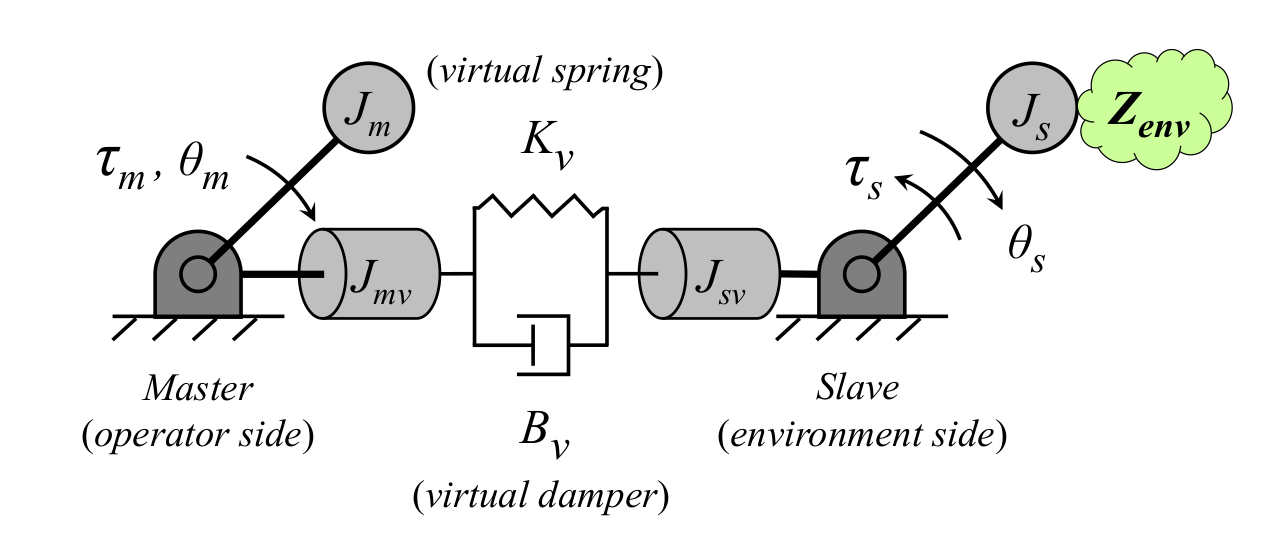
\includegraphics[width=0.7\linewidth]{Images/spring_damper_inertia_system}
	\caption{Spring-damper-inertia system with virtual parameters.}
	\label{fig:springdamperinertiasystem}
\end{figure}


The inertia-spring-damping system is shown in Fig.\ref{fig:springdamperinertiasystem}: the master and the slave have the real inertia $ J_m $ and $ J_s $ and the virtual ones $ J_{mv} $ and $ J_{sv} $. Master and slave are interconnected with the virtual damper $ B_v $ and the virtual spring $ K_v $.

The dynamic equation of the system are:
\begin{align}
	(J_m + J_{mv})\ddot{\theta}_m + B_v (\dot{\theta}_m - \dot{\theta}_s) + K_v(\theta_m - \theta_s) &= \tau_m \\
	(J_s + J_{sv})\ddot{\theta}_s + B_v (\dot{\theta}_s - \dot{\theta}_m) + K_v(\theta_s - \theta_m) &= - \tau_s 
\end{align}
and, in frequency domain:
\begin{align}
	(J_m + J_{mv}) s^2 \theta_m + (B_v s + K_v) (\theta_m - \theta_s) &= \tau_m \\
	(J_s + J_{sv}) s^2 \theta_s + (B_v s + K_v) (\theta_s - \theta_m) &= - \tau_s 
\end{align}

The virtual parameters are considered elements of the controller. For this aim the equations above are rearranged:
\begin{align}
	J_m s^2 \theta_m &= \tau_m - (B_v s + K_v) (\theta_m - \theta_s) - J_{mv} s^2 \theta_m \\
	J_s s^2 \theta_s &= - \tau_s - (B_v s + K_v) (\theta_s - \theta_m) - J_{sv} s^2 \theta_s \\
\end{align}
where the external torques are action and reaction forces of the human and the environment.

The block diagram of the proposed control system is constructed as shown in Fig.\ref{fig:blockdiagram}\footnote{Delay time in communication channel is not considered in the reference paper \cite{trakarnchaiyo2017vibration}.}.

\begin{figure}
	\centering
	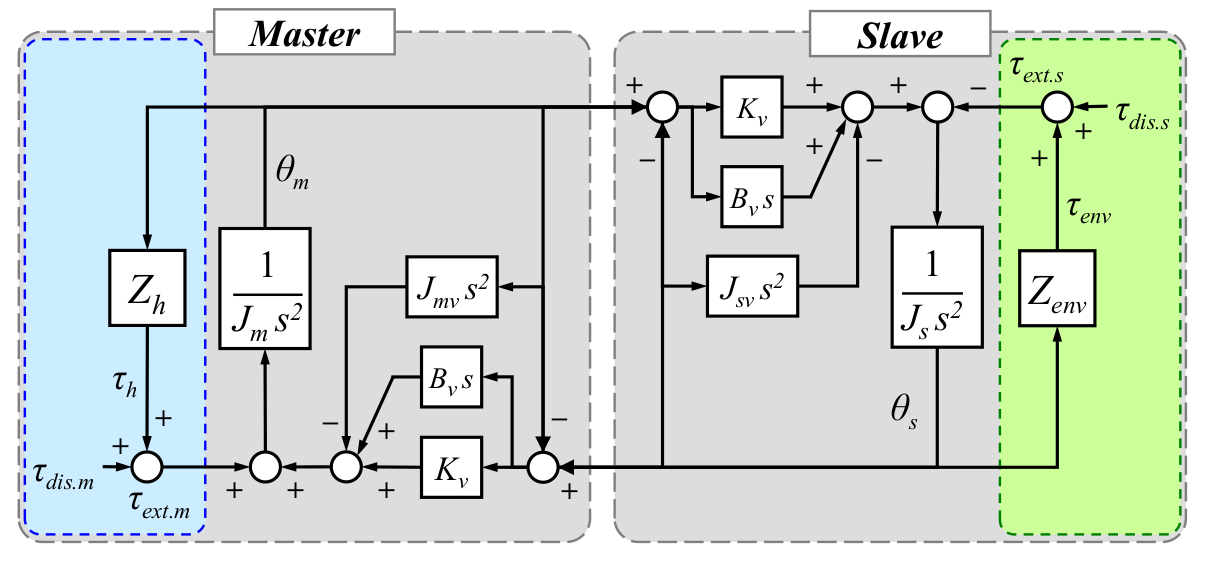
\includegraphics[width=0.7\linewidth]{Images/Block_diagram}
	\caption[block_diagram]{Block diagram of the bilateral control system.}
	\label{fig:blockdiagram}
\end{figure}

A bilateral control can be represented by a 2x2 matrix, called \emph{hybrid matrix}:
\begin{equation}
	\begin{bmatrix}
	\tau_m \\ \theta_s
	\end{bmatrix} = 
	\begin{bmatrix}
	H_{11} & H_{12} \\
	H_{21} & H_{22}
	\end{bmatrix}
	\begin{bmatrix}
	\theta_m \\ - \tau_s
	\end{bmatrix}
	\label{hybrid_matrix}
\end{equation}
and every $ H_{ij} $ is an hybrid parameter.

In particular:
\begin{align}
	H_{11} &= \frac{1}{Z_s}[Z_m Z_s - (B_v s + K_v)^2] \\
	H_{12} &= -\frac{1}{Z_s}[B_v s + K_v] \\
	H_{21} &= \frac{1}{Z_s}[B_v s + K_v] \\
	H_{22} &= \frac{1}{Z_s} 
\end{align}
where:
\begin{align}
	Z_m &= (J_m + J_{mv}) s^2 + B_v s + K_v \\
	Z_s &= (J_s + J_{sv}) s^2 + B_v s + K_v
\end{align}

The system should achieve two conditions:
\begin{itemize}
	\item the position of both sides should be the same;
	\item the law of action-reaction should hold;
\end{itemize}
represented by the \emph{transparency condition}:
\begin{align}
	\tau_m = \tau_s \\
	\theta_m = \theta_s
	\label{transparencY_condition}
\end{align}
is expressed in terms of transmitted impedance $ Z_t $, which is transferred to the human, and environment impedance $ Z_{env} $:
\begin{equation}
	\frac{\tau_m}{\theta_m} = Z_t = Z_{env} = \frac{\tau_s}{\theta_s}
\end{equation}

The relationship between the transmitted and environment impedance comes from the hybrid matrix of \eqref{hybrid_matrix}:
\begin{equation}
	Z_t = \big(\dfrac{-H_{12} H_{21}}{1 + H_{22} Z_{env}}\big)Z_{env} + H_{11}
\end{equation}
and, to achieve the perfect transparency condition shown in \eqref{transparencY_condition}, the hybrid parameters should be derived as:
\begin{equation}
	\begin{bmatrix}
	\tau_m \\ \theta_s
	\end{bmatrix} = 
	\begin{bmatrix}
	0 & -1 \\ 1 & 0
	\end{bmatrix}
	\begin{bmatrix}
	\theta_m \\ -\tau_s
	\end{bmatrix}
\end{equation}

The performances of a teleoperation are evaluated in \emph{free} and \emph{contact} motion. For free motion the external torque on the slave is usually equal to zero, and hence the only parameters affecting the transparency are $ H_{11} $ and $ H_{21} $. For contact motion, instead, all the hybrid parameters affect the performance.

\subsection{Parameter selection and design}\label{ParamSelect} 

The system is assumed to be disturbed by external vibration noise from the environment. We want to know how the slave position is affected by the external noise. This analysis can be achieved inspecting the hybrid parameter $ H_{22} $, representing how the position responds to external torque:
\begin{equation}
	\dfrac{\theta_s}{\tau_{ext}} = \dfrac{1}{(J_s + J_{sv}) s^2 + B_v s + K_v}
	\label{H_22}
\end{equation}

The virtual parameter in \eqref{H_22} are determined from the second-order characteristic equation of the system:
\begin{equation}
%	s^2 + (g_1 + g_2) s + (g_1 \cdot g_2) = 0
	(s + g_1)(s + g_2) = 0
	\label{charact_equation}
\end{equation}  
where the poles $ g_1 $ and $ g_2 $ represent the cut-off frequencies of the system for disturbance suppression purpose.

We can determine the virtual parameters comparing the characteristic equation of \eqref{H_22} with \eqref{charact_equation}.

The operator should feel the reflecting force from the environment vividly. Assuming for a moment we do not care about the vibration suppression, for the proposed control the system can achieve a large transparency with high spring stiffness $ K_v $ and a damping $ B_v \rightarrow 0 $. 

It is clear that the value of spring stiffness $ K_v $ has an important influence on the transparency of the system: we want to choose it beforehand and the other virtual parameters will be calculated accordingly.
The virtual damping coefficient $ B_v $:
\begin{equation}
	\frac{B_v}{K_v} = \frac{g_1 + g_2}{g_1 \cdot g_2} \quad \Rightarrow \quad B_v = \frac{g_1 + g_2}{g_1 \cdot g_2} K_v
\end{equation}
and, in the same fashion, the virtual inertia $ J_{sv} $:
\begin{equation}
	J_{sv} = \frac{1}{g_1 \cdot g_2} K_v - J_s
\end{equation}

The spring stiffness, as said before, influences the behavior of the system. Choosing it properly we can obtain:
\begin{itemize}
	\item \textbf{rigid coupling}, with high stiff spring, obtaining an high transparency;
	\item \textbf{spring coupling}, when the value of the stiffness is low.
\end{itemize}

In other words we can use the spring stiffness to regulate the \emph{compliance} of the system.